% EF5342 Week 10 — Commercial Banks and Investment Banks
% Beamer conversion from week10_Banks.pptx (60 source slides -> 40 frames).
% Compile: pdflatex week10_Banks.tex
% Each frame carries a [src: ...] comment mapping back to source slides
% (the content-coverage checklist; S = section divider slide in the pptx).
\documentclass[aspectratio=169]{beamer}
\usepackage{../ef5342}

\title{EF5342 Financial Systems, Markets and Instruments}
\subtitle{Week 10 --- Commercial Banks and Investment Banks}
\author{Prof.\ Weikai Li}
\institute{City University of Hong Kong}
\date{Semester B 2026--2027}

\begin{document}

% ============ COMMERCIAL BANKS ============

% [src: 1]
% Title-slide background art (slide01_img.jpg) dropped — decorative.
\begin{frame}
\titlepage
\end{frame}

% [src: 2]
\begin{frame}{Overview}
\begin{columns}
\begin{column}{0.48\textwidth}
\textbf{Commercial banks}
\begin{itemize}
  \item Commercial bank activities
  \item Structure and trends of the US banking industry
  \item Regulation of commercial banks
\end{itemize}
\end{column}
\begin{column}{0.48\textwidth}
\textbf{Investment banks}
\begin{itemize}
  \item Industry structure and competitive dynamics
  \item Investment bank activities
  \item Regulation of investment banks
\end{itemize}
\end{column}
\end{columns}
\end{frame}

% [src: 3]
\begin{frame}{Commercial Banks}
A bank \textbf{intermediates between the borrower and the lender}: instead of raising capital directly, a company can borrow from a bank. Banks matter especially in markets where bond and equity markets are less developed.
\begin{itemize}
  \item \textbf{Screen and monitor} borrowers --- ensures capital is put to good, productive use
  \item \textbf{Maturity intermediation} --- borrow short-term to fund long-term assets
  \item Play a key role in the \textbf{transmission of monetary policy}
\end{itemize}
\vspace{0.3em}
Banks are heavily regulated to protect against disruptions to the services they perform.
\end{frame}

% [src: 4, 5, 6]
\begin{frame}{Multiple Roles of Banks}
\begin{description}
  \item[Lender] Banks originate and hold loans (mortgages, business loans, consumer credit, syndicated facilities)
  \item[Borrower] Banks borrow from depositors, other banks (interbank market), central banks (discount window), or wholesale markets (repos, commercial paper, bonds)
  \item[Liquidity providers] Lines of credit that firms can draw when needed
  \item[Credit enhancement] Letters of credit guaranteeing that a buyer's payment to a seller will be received on time and for the correct amount
  \item[Payment channel] The backbone of payment systems --- checks, wires (SWIFT, Fedwire), cards
  \item[Conduit for monetary policy] Banks transmit central bank policy --- lending rates, reserve requirements, and open-market effects flow through banks to the economy
  \item[Trustees] Act as trustees in structured finance --- managing collateral, enforcing terms, distributing cash flows (securitizations, indenture trustees)
  \item[Custody agents] Safeguard assets --- holding securities, cash, or instruments for clients (institutional investors, mutual funds, central counterparties)
\end{description}
\note{Monetary policy transmission: central banks adjust the policy rate (fed funds rate in the US, deposit facility rate at the ECB); banks pass this through to loan and deposit rates. Lower policy rates mean lower loan and deposit rates; lower deposit rates reduce the incentive to save, boosting consumption.}
\end{frame}

% [src: 7]
\begin{frame}{Historical Development of the US Banking Industry}
\begin{figure}
\centering
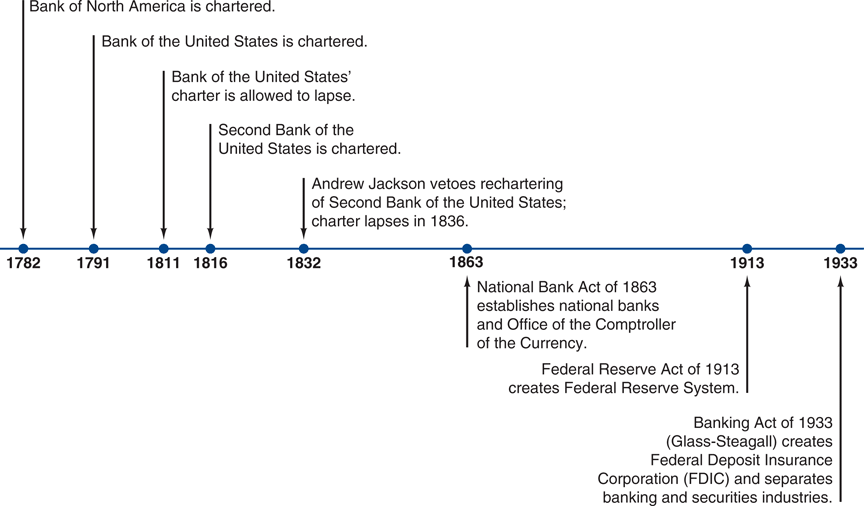
\includegraphics[height=0.58\textheight,keepaspectratio]{figures/slide07_img.png}
\caption{Timeline of the early history of commercial banking in the United States}
\end{figure}
\note{Key milestones from the Revolutionary era through the Great Depression: from ad hoc war-financed banks to a structured national banking system, the rise and fall of early central banks, a permanent federal framework, and Depression-era reforms.}
\end{frame}

% [src: 8, 9]
\begin{frame}{Balance Sheets: Commercial Banks vs.\ Nonfinancial Firms}
A bank's balance sheet is typically the \textbf{opposite} of a non-financial firm's: a bank's \emph{assets} are loans and its \emph{liabilities} are deposits; a non-financial firm's assets are deposits and its liabilities are loans.
\begin{center}
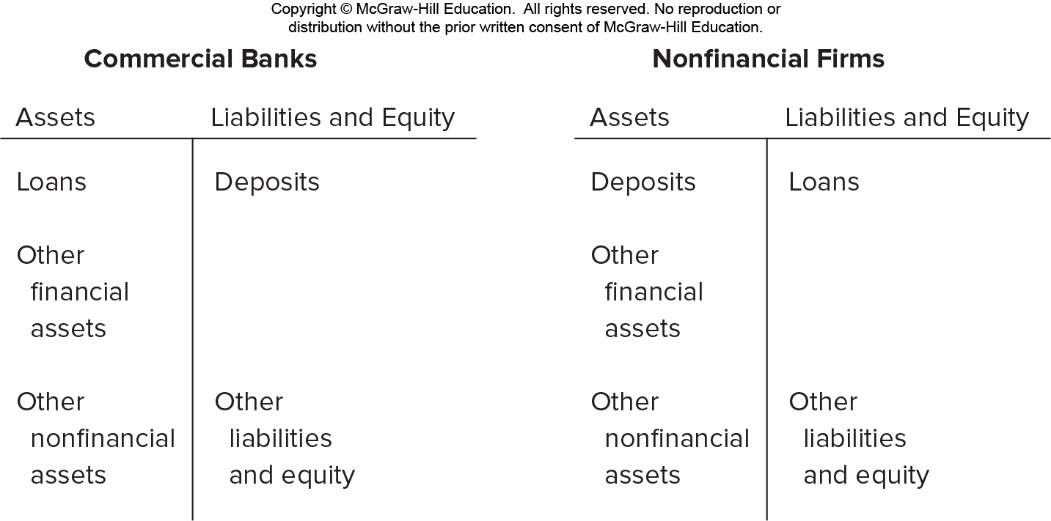
\includegraphics[height=0.28\textheight,keepaspectratio]{figures/slide08_img.jpg}
\hspace{0.5em}
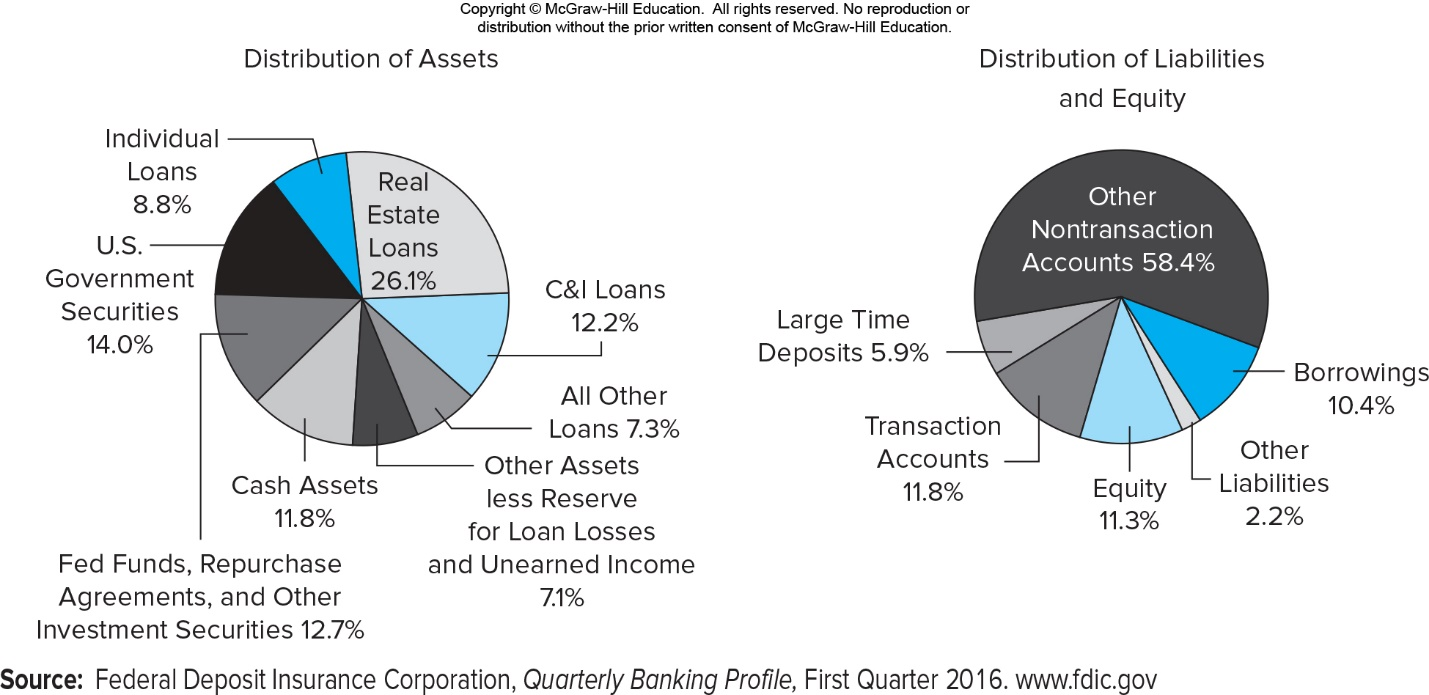
\includegraphics[height=0.28\textheight,keepaspectratio]{figures/slide09_img.jpg}
\end{center}
\end{frame}

% [src: 10, 11]
\begin{frame}{Commercial Bank Assets}
\begin{columns}
\begin{column}{0.54\textwidth}
\textbf{Loans} generate the most revenue:
\begin{itemize}\small
  \item Commercial \& industrial (C\&I) loans are \emph{declining} --- nonbank lending substitutes such as commercial paper
  \item Mortgages (residential real estate) and consumer loans (credit cards, auto, personal) have increased in importance over the long term
\end{itemize}
\textbf{Other assets:}
\begin{itemize}\small
  \item \textbf{Investment securities}: funds lent to other banks, or investments in other debt/equity instruments
  \item \textbf{Cash assets}: held to meet reserve requirements and provide liquidity
  \item \textbf{Other assets}: premises and equipment, other real estate owned, etc.
\end{itemize}
\end{column}
\begin{column}{0.44\textwidth}
\begin{figure}
\centering
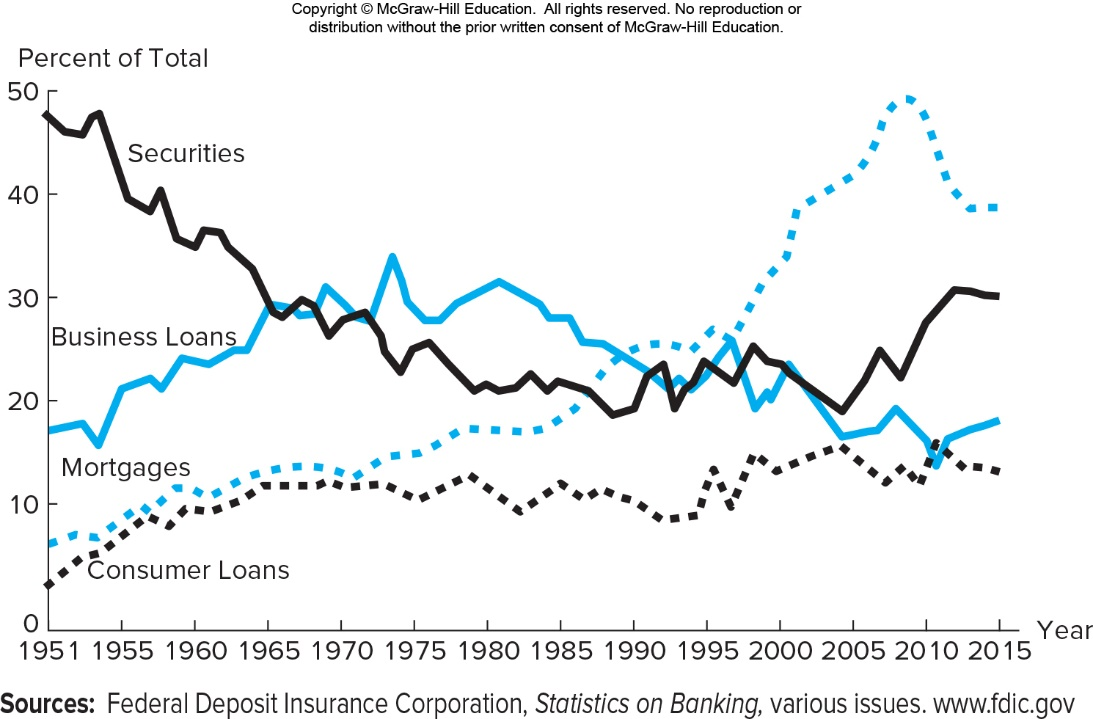
\includegraphics[height=0.46\textheight,keepaspectratio]{figures/slide11_img.jpg}
\end{figure}
\end{column}
\end{columns}
\note{Mortgages and consumer loans are rising, while business lending is declining.}
\end{frame}

% [src: 12, 13]
\begin{frame}{Commercial Bank Liabilities and Equity}
\begin{description}
  \item[Liabilities] Interest-bearing deposits (savings), non-interest-bearing deposits (current accounts), time deposits (fixed deposits), and other borrowings (fed funds, interbank borrowing, repos). Liabilities usually have \textbf{shorter maturities and are more liquid} than bank assets --- banks face \textbf{maturity mismatch and liquidity risk}: if short-term rates rise suddenly, funding costs rise while interest income from assets stays the same
  \item[Equity] Common and preferred stock, surplus (additional paid-in capital), and retained earnings. Regulators require \textbf{minimum equity capital} as a buffer against losses. If deposit funding is cheap, banks keep equity at the minimum --- putting funds to maximum use to earn profits, at the cost of exposure to insolvency if market conditions worsen suddenly
\end{description}
\end{frame}

% [src: 14]
\begin{frame}{Off-Balance Sheet Activities}
\textbf{Off-balance sheet (OBS) activities} are commitments or exposures that do not appear as assets or liabilities on the balance sheet under standard accounting rules. They generate fee income, service clients, manage risk, or create contingent obligations without immediately using balance sheet capacity. Major categories:
\begin{description}
  \item[Unused loan commitments] Promises to lend in the future (e.g., revolving credit facilities)
  \item[Letters of credit] Bank charges a fee for guaranteeing a firm's future payment; if the firm defaults, the bank adds the item to liabilities
  \item[Loans sold (securitization)] The bank may have to buy back loans when quality deteriorates (clawback provisions in the subprime mortgage crisis)
  \item[Derivative contracts] When speculative bets turn out wrong, the bank could face insolvency
\end{description}
\note{The bank's letter of credit guarantees payment to the seller as long as agreed-upon delivery conditions have been met --- if the good or service is provided and the buyer cannot pay, the bank pays on the buyer's behalf.}
\end{frame}

% ============ STRUCTURE AND TRENDS ============

% [src: 15]
\section{Structure and Trends of the US Banking Industry}

% [src: 16]
\begin{frame}{Number of Insured Commercial Banks in the United States, 1934--2022}
\begin{figure}
\centering
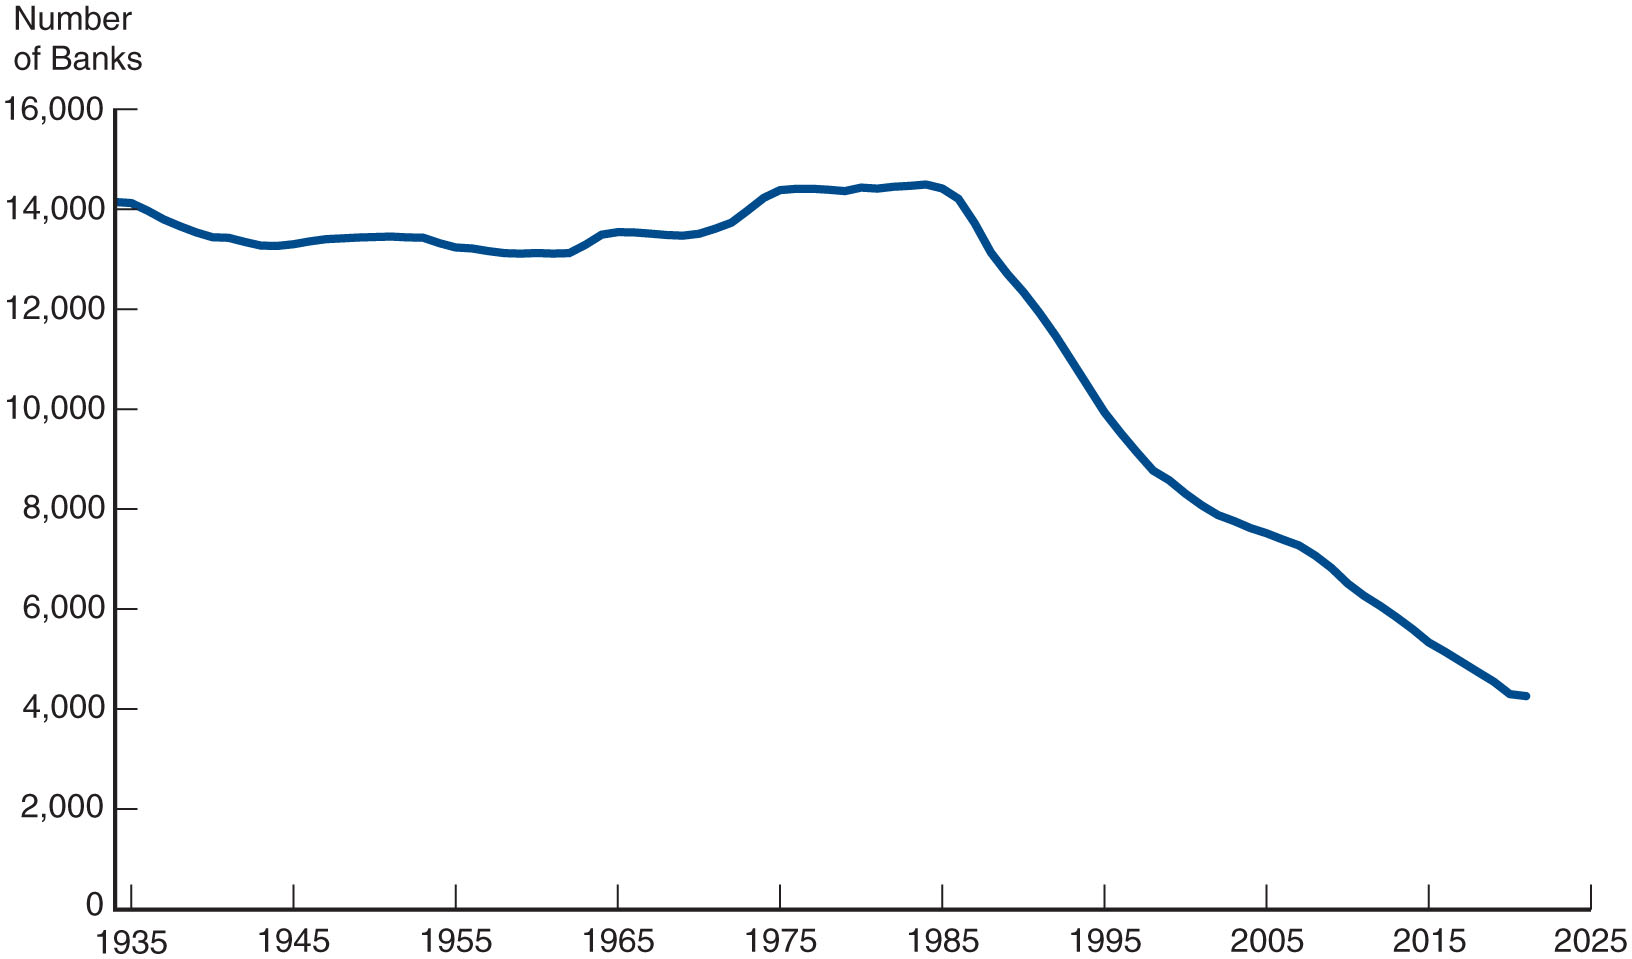
\includegraphics[height=0.58\textheight,keepaspectratio]{figures/slide16_img.jpg}
\end{figure}
\begin{center}
\small Source: FDIC, \href{https://www5.fdic.gov/hsob/HSOBRpt.asp}{HSOB} (chart vintage: year-end 2022).\\
Current total: 4{,}238 FDIC-insured institutions as of Q2 2026 (FDIC QBP) --- the consolidation trend continues.
\end{center}
\end{frame}

% [src: 17]
\begin{frame}{Size Distribution of US Banking Institutions}
\begin{table}
\centering
\small
\begin{tabular}{lrrrr}
\toprule
\textbf{Assets} & \textbf{Number of banks} & \textbf{Share of banks (\%)} & \textbf{Share of assets held (\%)} \\
\midrule
Less than \$100 million & 543 & 12.8 & 0.1 \\
\$100 million--\$1 billion & 2{,}647 & 62.5 & 3.9 \\
\$1 billion--\$10 billion & 890 & 21.0 & 9.4 \\
\$10 billion--\$250 billion & 140 & 3.3 & 22.9 \\
More than \$250 billion & 18 & 0.4 & 63.7 \\
Total & 4{,}238 & 100.0 & 100.0 \\
\bottomrule
\end{tabular}
\end{table}
\begin{center}
\small FDIC-insured commercial banks and savings institutions, as of Q2 2026 (FDIC QBP; total assets \$26.5 trillion) --- \href{https://www.fdic.gov/analysis/quarterly-banking-profile/}{Quarterly Banking Profile}
\end{center}
\end{frame}

% [src: 18]
\begin{frame}{Restrictions on Branching}
\textbf{Branching restrictions (McFadden Act of 1927)} --- very anti-competitive:
\begin{itemize}
  \item Explicit prohibition on \textbf{interstate branching}: national banks could branch only within the state where headquartered
\end{itemize}
\vspace{0.2em}
\textbf{Responses to the restrictions:}
\begin{description}
  \item[Bank holding companies (BHCs)] Allowed purchases of banks outside the state; the Fed allowed BHCs a wider scope of activities; BHCs are the dominant corporate form ($\approx$97\% of US banking-industry assets are held inside holding-company structures, FDIC Q2 2026)
  \item[Automated teller machines (ATMs)] Not considered a branch of the bank, so networks were allowed
\end{description}
\note{BHCs are corporate entities that own or control one or more FDIC-insured depository institutions but do not themselves directly accept deposits or make loans; the holding company oversees subsidiary banks and often nonbank affiliates.}
\end{frame}

% [src: 19, 20, 21]
\begin{frame}{Bank Consolidation and Nationwide Banking}
\begin{columns}
\begin{column}{0.52\textwidth}
\textbf{Why consolidation?}
\begin{itemize}\small
  \item Loophole mining reduced the effectiveness of branching restrictions; development of super-regional banks
  \item Economies of scale (increased with information technology); economies of scope in using data for pricing, new products --- birth of large, complex banking organizations (LCBOs)
  \item \textbf{Riegle-Neal Act of 1994}: allows full interstate branching --- facilitating consolidation, larger institutions, and competition, but raising systemic-risk and local-service concerns
  \item \textbf{Future}: more like other countries, but not quite --- several thousand (not several hundred) banks; only half of small banks remain, large banks expected to double in number
\end{itemize}
\end{column}
\begin{column}{0.44\textwidth}
\textbf{Is it a good thing?}
\begin{itemize}\small
  \item[\textbf{Cons:}]
  \item Fear of decline of small banks and small-business lending
  \item Rush to consolidation may increase risk taking
  \item[\textbf{Pros:}]
  \item Increases competition and efficiency
  \item Greater diversification of bank loan portfolios lessens the likelihood of failures
\end{itemize}
\end{column}
\end{columns}
\end{frame}

% [src: 22]
\begin{frame}{Largest Banks in the United States}
Top 10 US banks by total assets (June 30, 2026, FDIC Call Reports):
\begin{table}
\centering
\footnotesize
\begin{tabular}{clr}
\toprule
\textbf{\#} & \textbf{Bank} & \textbf{Total assets} \\
\midrule
1 & JPMorgan Chase Bank, N.A. & \$4.09 trillion \\
2 & Bank of America, N.A. & \$2.65 trillion \\
3 & Citibank, N.A. & \$1.98 trillion \\
4 & Wells Fargo Bank, N.A. & \$1.91 trillion \\
5 & Goldman Sachs Bank USA & \$0.76 trillion \\
6 & U.S.\ Bank, N.A. & \$0.71 trillion \\
7 & Capital One, N.A. & \$0.66 trillion \\
8 & PNC Bank, N.A. & \$0.61 trillion \\
9 & Truist Bank & \$0.55 trillion \\
10 & BNY Mellon, N.A. & \$0.43 trillion \\
\bottomrule
\end{tabular}
\end{table}
\end{frame}

% [src: 23]
\begin{frame}{Bank Performance Measures}
\begin{description}
  \item[Interest rate spread] Difference between lending and deposit rates
  \item[Net interest margin] Interest income minus interest expense, divided by earning assets
  \item[Net non-interest margin] Non-interest income minus non-interest expense, divided by earning assets (trading profits, service charges on deposits, credit card fees)
  \item[Net charge-offs] Percentage of loans written off as uncollectable
  \item[Nonperforming loan (NPL)] Borrowed money on which the debtor has not made scheduled payments for at least 90 days
  \item[ROA / ROE] Net income divided by assets / by equity
\end{description}
\vspace{0.2em}
Bank profitability declines and charge-offs rise during economic recessions.
\end{frame}

% [src: 24, 25, 26, 27]
\begin{frame}{Bank Performance over Time}
\begin{center}
\begin{columns}
\begin{column}{0.48\textwidth}
\centering
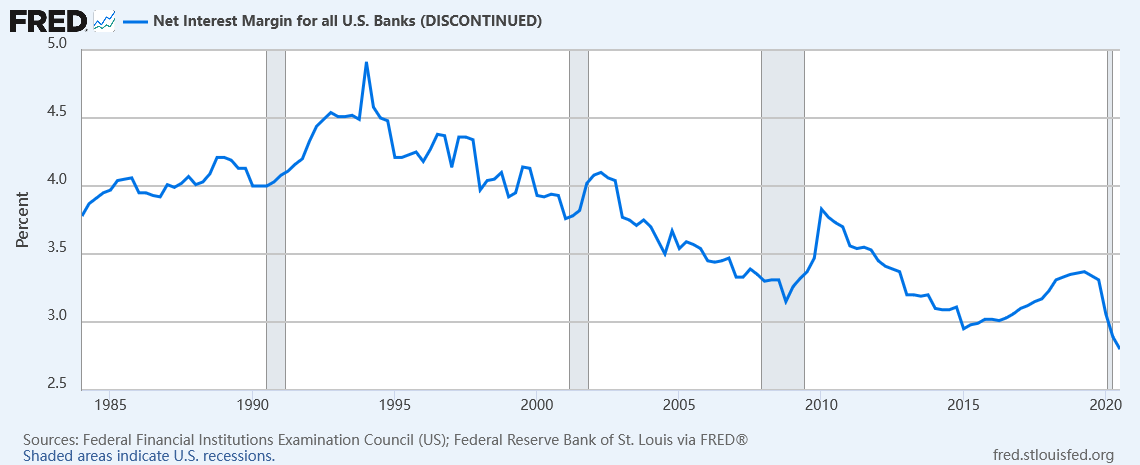
\includegraphics[width=0.94\linewidth,keepaspectratio]{figures/slide24_img_flat.png}\\
{\scriptsize Net interest margin}
\end{column}
\begin{column}{0.48\textwidth}
\centering
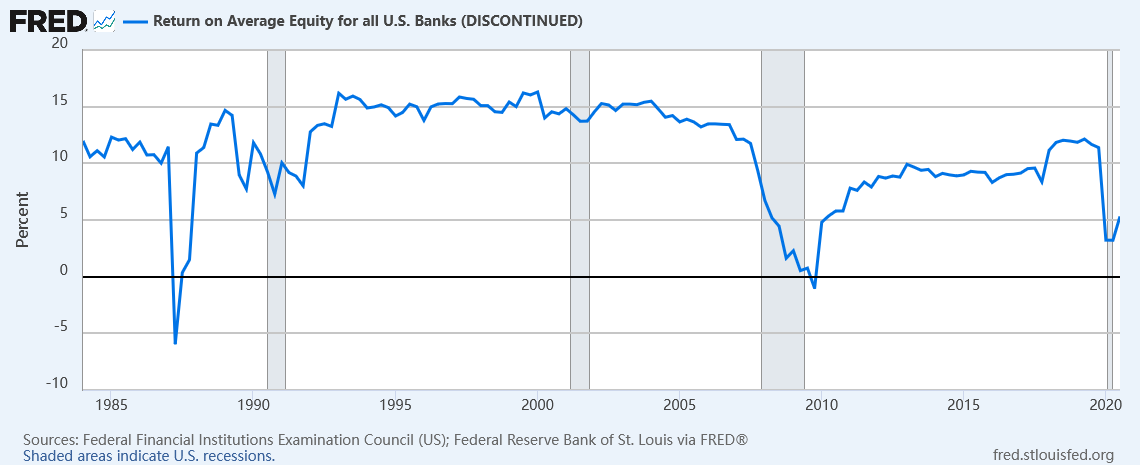
\includegraphics[width=0.94\linewidth,keepaspectratio]{figures/slide25_img_flat.png}\\
{\scriptsize Return on assets}
\end{column}
\end{columns}
\begin{columns}
\begin{column}{0.48\textwidth}
\centering
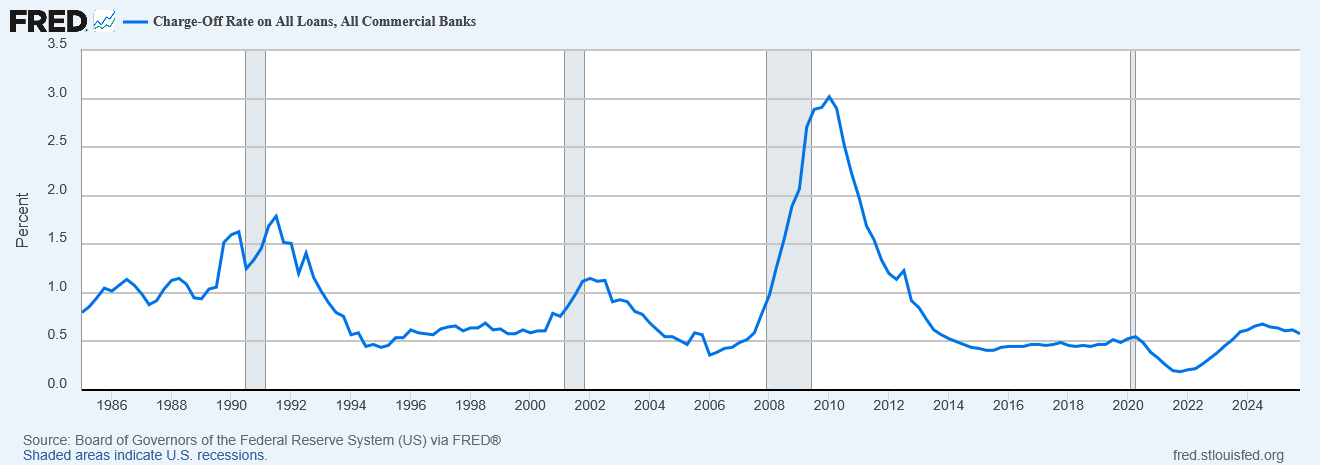
\includegraphics[width=0.94\linewidth,keepaspectratio]{figures/slide26_img_flat.png}\\
{\scriptsize Charge-off rate}
\end{column}
\begin{column}{0.48\textwidth}
\centering
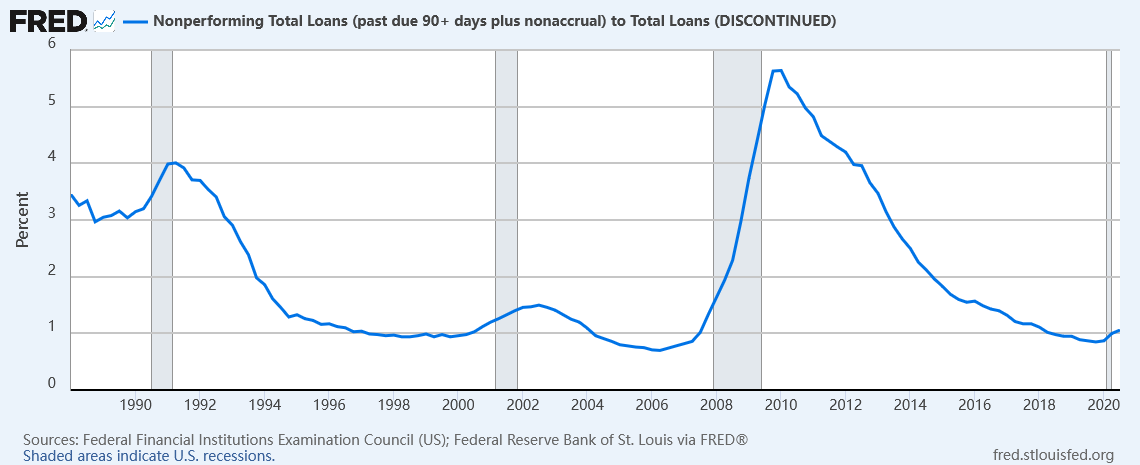
\includegraphics[width=0.94\linewidth,keepaspectratio]{figures/slide27_img_flat.png}\\
{\scriptsize Nonperforming loans}
\end{column}
\end{columns}
\small Source: Federal Reserve Bank of St. Louis
\end{center}
\note{Bank NIM rose with the 2022--23 tightening cycle and has since plateaued around 3.3\% (FDIC QBP Q2 2026: 3.32\%). On the ROA and charge-off charts, the spike around the 1980s--90s reflects the S\&L crisis (federalreservehistory.org).}
\end{frame}

% ============ BANK REGULATION ============

% [src: 28]
\section{Regulation of the Banking Industry}

% [src: 29]
\begin{frame}{What Are the Major Risks Banks Face?}
Commercial banks face risks that can threaten their solvency, profitability, reputation, and operational continuity:
\begin{enumerate}
  \item \textbf{Credit risk} --- borrowers defaulting on loans or other credit exposures
  \item \textbf{Market risk \& interest rate risk in the banking book} --- losses from adverse moves in interest rates, equity prices, FX, or commodities (trading books, asset--liability mismatches)
  \item \textbf{Liquidity risk} --- inability to meet obligations without unacceptable losses (funding or market liquidity)
  \item \textbf{Operational risk (incl.\ cyber \& IT)} --- losses from inadequate or failing processes, people, systems, or external events
  \item \textbf{Regulatory \& compliance risk} --- failure to meet laws, rules, or standards, leading to fines, restrictions, or forced changes
\end{enumerate}
\end{frame}

% [src: 30]
\begin{frame}{US Banking Regulations}
\begin{description}
  \item[FDIC] Insures deposits of commercial banks --- \$250{,}000 per bank account; examines and supervises about 4{,}000 banks for safety and soundness. \emph{(Video: importance of the FDIC for financial stability)}
  \item[Dual banking system] Banks can be nationally or state-chartered: the Office of the Comptroller of the Currency (OCC) charters and regulates national banks; state agencies charter and regulate state banks
  \item[Federal Reserve System] Regulatory power over nationally chartered banks and their holding companies, and state banks that opt into the Federal Reserve System
\end{description}
\end{frame}

% [src: 31, 32]
\begin{frame}{International Banking Regulations: Basel III}
\textbf{Basel III} --- a comprehensive international framework from the Basel Committee on Banking Supervision (BCBS) to strengthen global banking resilience: more and better capital, less leverage, better liquidity management, enhanced risk coverage.
\begin{description}
  \item[Pillar 1: Minimum capital requirements] Higher quantity and quality of capital, emphasizing \textbf{Common Equity Tier 1 (CET1)}; minimum CET1 ratio raised to \textbf{4.5\% of risk-weighted assets}
  \item[Pillar 2: Supervisory review] Banks assess their overall risk profile; supervisors review it (SREP) --- promoting stronger governance, stress testing, and risk management
  \item[Pillar 3: Market discipline] Detailed, standardized public disclosures on capital, risk exposures, RWAs, leverage, liquidity, and remuneration --- so markets can assess bank soundness
\end{description}
\vspace{0.2em}
The most significant overhaul of banking regulation since the 1930s.
\end{frame}

% ============ INVESTMENT BANKS ============

% [src: 33]
\section{Investment Banks}

% [src: 34]
\begin{frame}{Investment Banks (IBs)}
Investment banking: financial intermediation services helping corporations, governments, and institutional investors \textbf{raise capital, execute strategic transactions, and manage financial risk}. Principal business lines:
\begin{description}
  \item[M\&A advisory] Buy-side and sell-side counsel on corporate transactions, valuations, and deal structures
  \item[Equity capital markets (ECM)] Underwriting and distributing IPOs, follow-on offerings, convertibles
  \item[Debt capital markets (DCM)] Underwriting investment-grade and high-yield bonds, leveraged loans, syndicated credit facilities
  \item[Sales \& trading] Intermediating client transactions and managing positions in equities and FICC
  \item[Research] Equity and credit analysis for institutional investors
\end{description}
\end{frame}

% [src: 35, 36]
\begin{frame}{Market Size and Industry Structure}
\begin{columns}
\begin{column}{0.50\textwidth}
\begin{center}
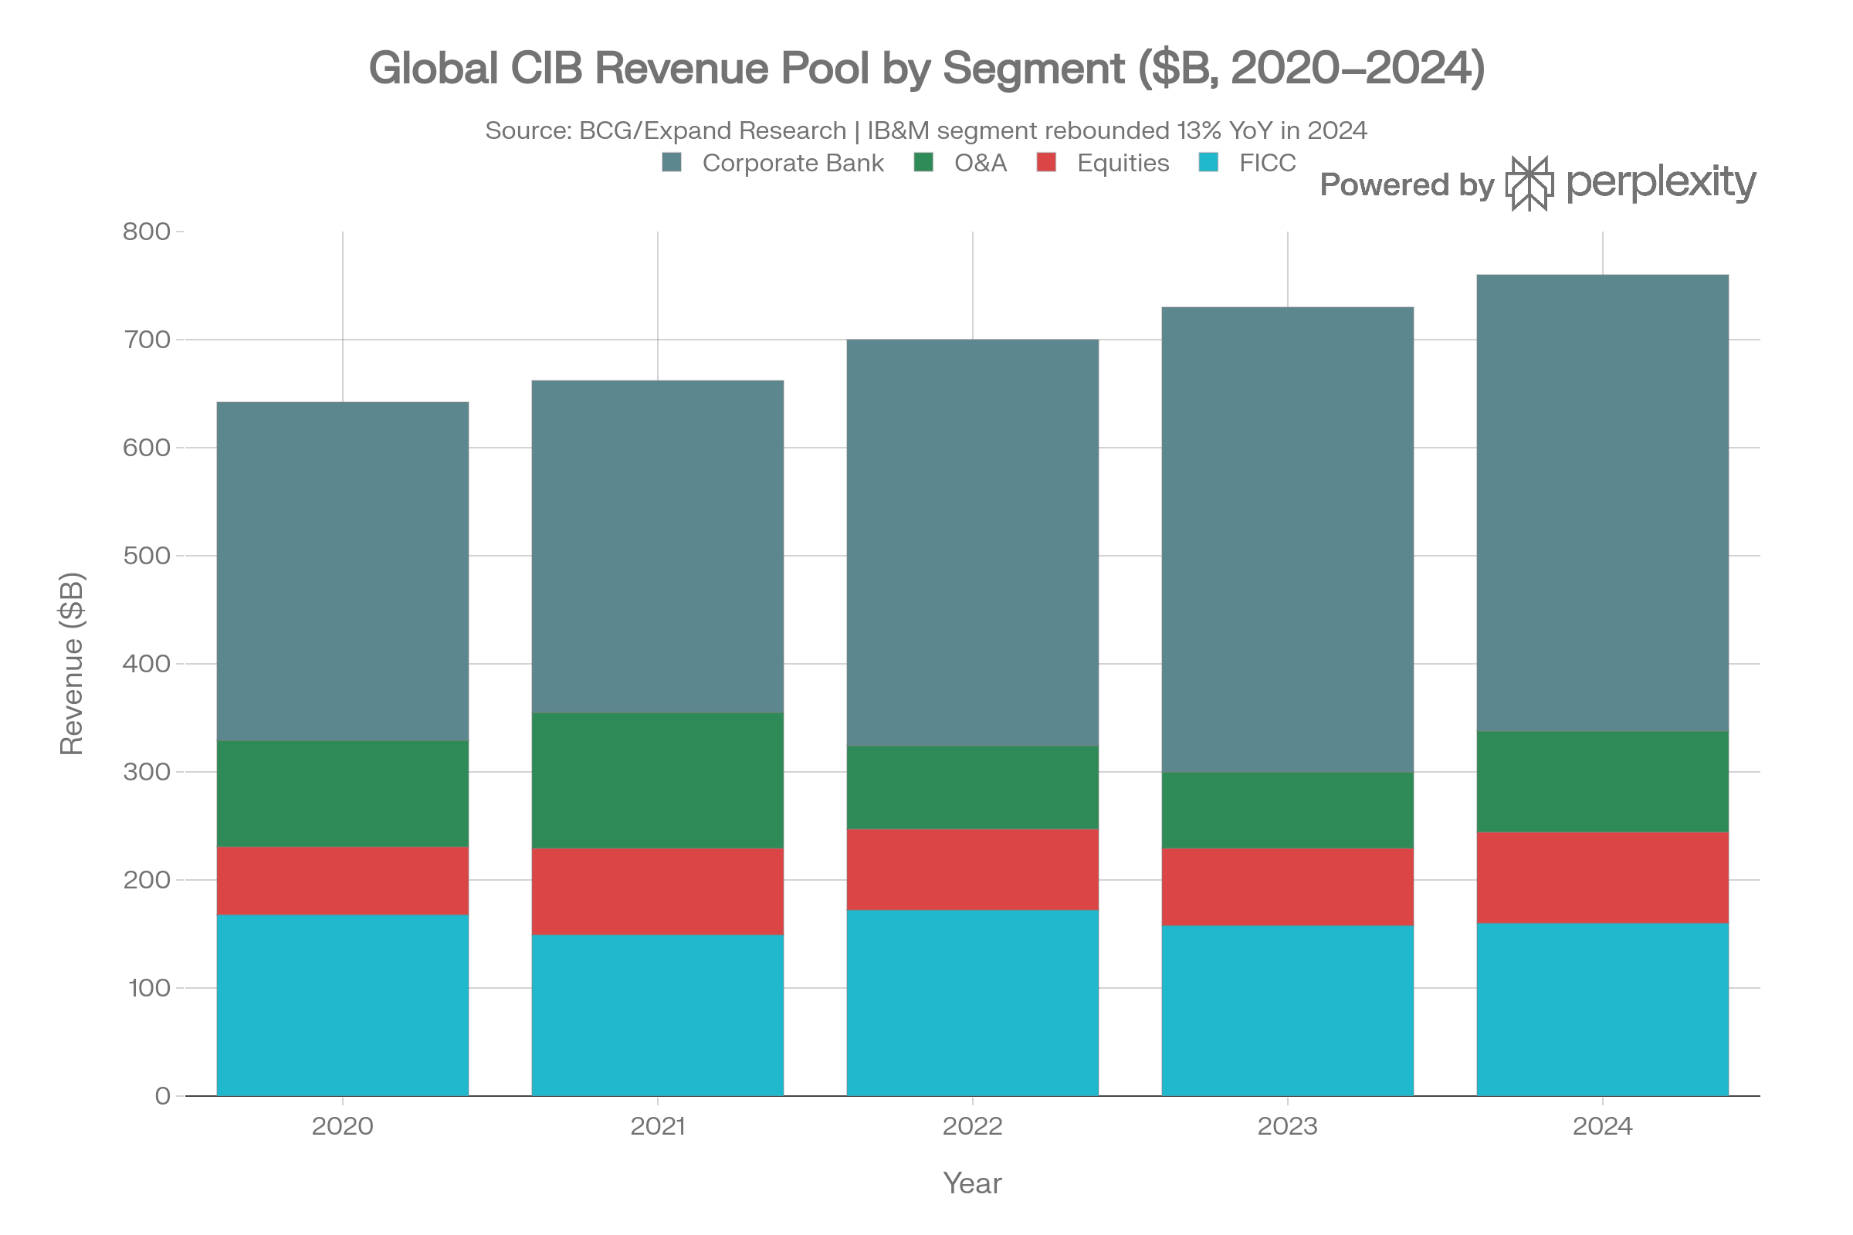
\includegraphics[height=0.40\textheight,keepaspectratio]{figures/slide35_img_flat.png}\\
{\scriptsize Global IB revenue trends}
\end{center}
\end{column}
\begin{column}{0.48\textwidth}
Investment banking is a \textbf{highly concentrated oligopoly}: per FT/LSEG league tables, YTD 2026 (H1 global IB fees \$78 billion, +14\% year-over-year), the top five US banks collectively dominate the global IB fee pool.
\begin{center}
\vspace{0.3em}
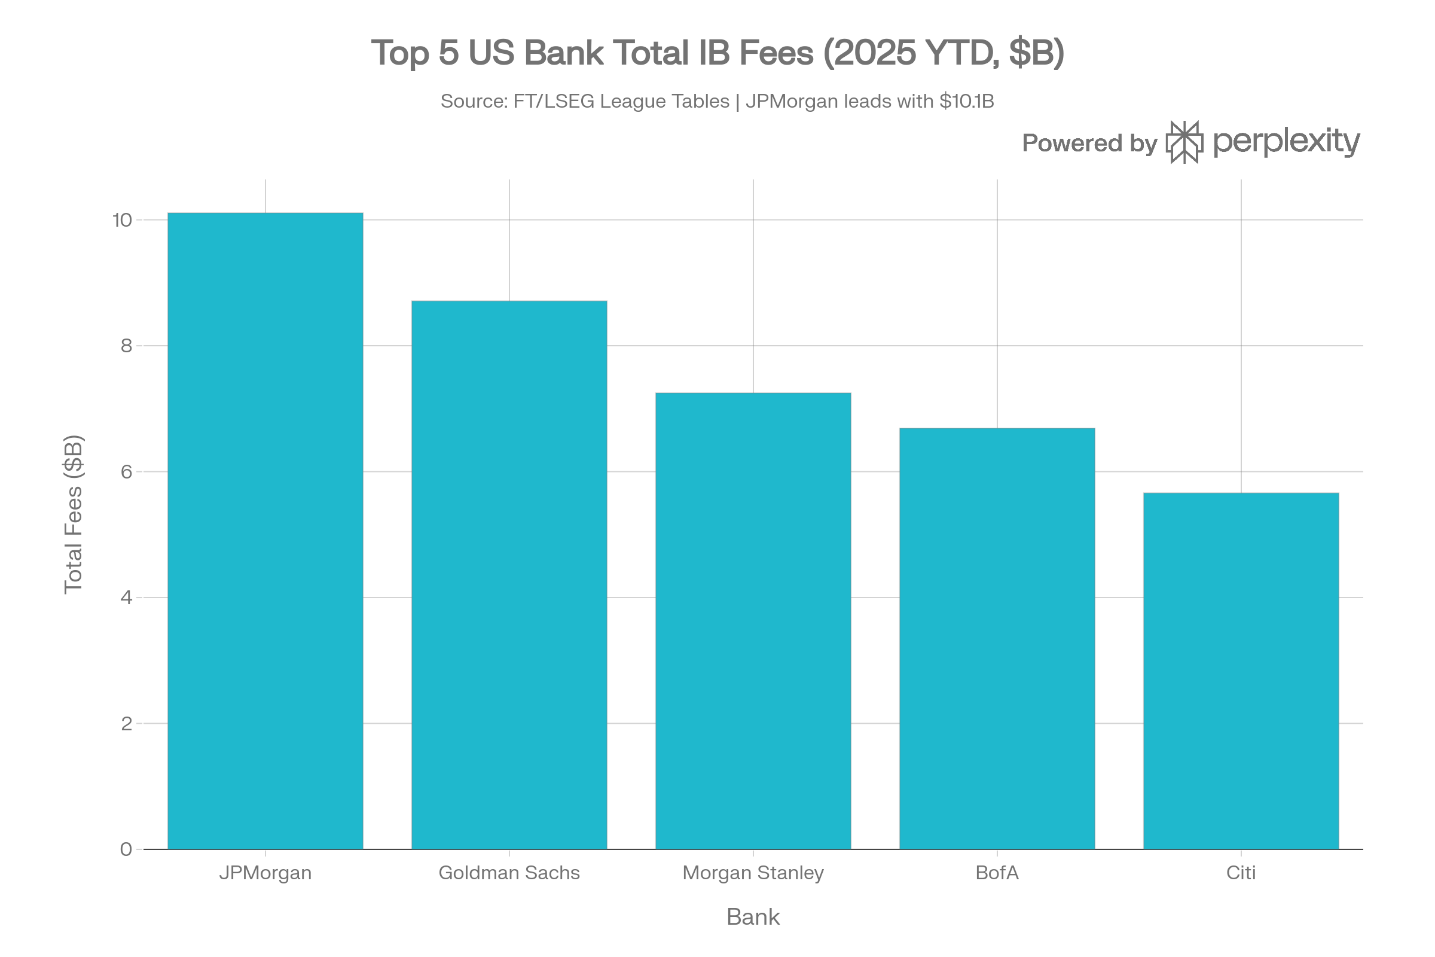
\includegraphics[height=0.40\textheight,keepaspectratio]{figures/slide36_img_flat.png}
\end{center}
\end{column}
\end{columns}
\end{frame}

% [src: 37]
\begin{frame}{Investment Banking Scorecard}
\begin{center}
\begin{columns}
\begin{column}{0.48\textwidth}
\centering
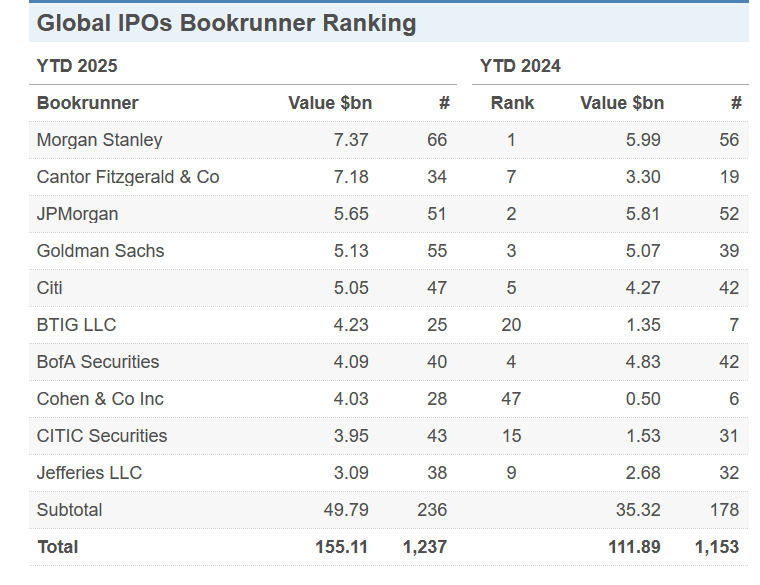
\includegraphics[height=0.36\textheight,keepaspectratio]{figures/slide37_img_flat.png}
\end{column}
\begin{column}{0.48\textwidth}
\centering
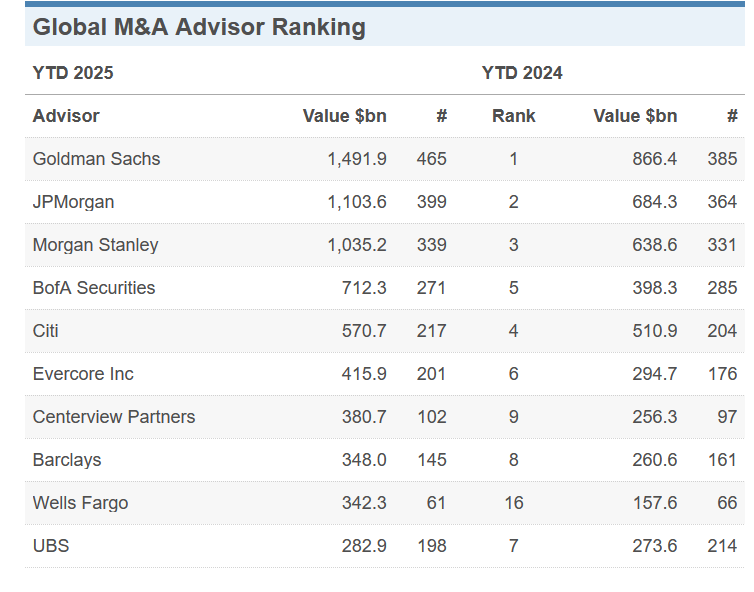
\includegraphics[height=0.36\textheight,keepaspectratio]{figures/slide37_img1_flat.png}
\end{column}
\end{columns}
\end{center}
\begin{center}
\small Source: \href{https://dealogic.com/investment-banking-scorecard/}{Dealogic Investment Banking Scorecard}
\end{center}
\end{frame}

% [src: 38]
\begin{frame}{Industry Structure: Firm Typology (1/2)}
\textbf{Bulge bracket banks} --- the designation derives from listing the largest underwriters first (in larger, ``bulging'' type) on tombstone announcements. As of 2026, eight firms qualify: JPMorgan, Goldman Sachs, Bank of America, Morgan Stanley, Citigroup, Barclays, UBS, and Deutsche Bank. Defining characteristics:
\begin{itemize}
  \item Global presence across 60+ countries and 100+ markets
  \item Full-service capability: M\&A, ECM, DCM, trading, research, asset management
  \item Massive balance sheets enabling multi-billion-dollar underwritings and bridge commitments
  \item Clients: Fortune 500 corporations, sovereign wealth funds, institutional investors
\end{itemize}
\end{frame}

% [src: 39]
\begin{frame}{Industry Structure: Firm Typology (2/2)}
\begin{description}
  \item[Elite boutiques] M\&A advisory without the bulge-bracket balance sheet --- Evercore, Lazard, Centerview Partners, Moelis, PJT Partners challenge bulge brackets for advisory mandates on landmark deals. Flat hierarchies, senior banker attention, and a conflict-free advisory model appeal to certain clients
  \item[Middle-market banks] Jefferies, Houlihan Lokey, William Blair, Piper Sandler --- serving companies in the \$50M--\$500M revenue range
  \item[Regional and specialty boutiques] Focus on specific geographies (Southwest US, Pacific Northwest) or sectors (healthcare, energy, technology); particularly active in transactions below \$100M and critical training grounds for early-career bankers
\end{description}
\end{frame}

% ============ INVESTMENT BANK ACTIVITIES ============

% [src: 40]
\section{Investment Bank Activities}

% [src: 41, 42]
\begin{frame}{Mergers \& Acquisitions Advisory}
\begin{columns}
\begin{column}{0.52\textwidth}
\begin{itemize}\small
  \item \textbf{Fees}: typically 1--2\% of deal value for smaller transactions, tapering to 0.1--0.5\% for mega-deals ($>$\$5B)
  \item \textbf{Buy-side vs.\ sell-side}: advising acquirers on identifying and valuing targets; advising targets on auction processes and defence
  \item \textbf{Fairness opinions}: independent valuations for boards facing conflicts of interest
  \item \textbf{Fairness-of-price analysis}: DCF models, LBO analysis, trading comparables, precedent transactions --- the core financial modeling toolkit
\end{itemize}
\end{column}
\begin{column}{0.46\textwidth}
\begin{figure}
\centering
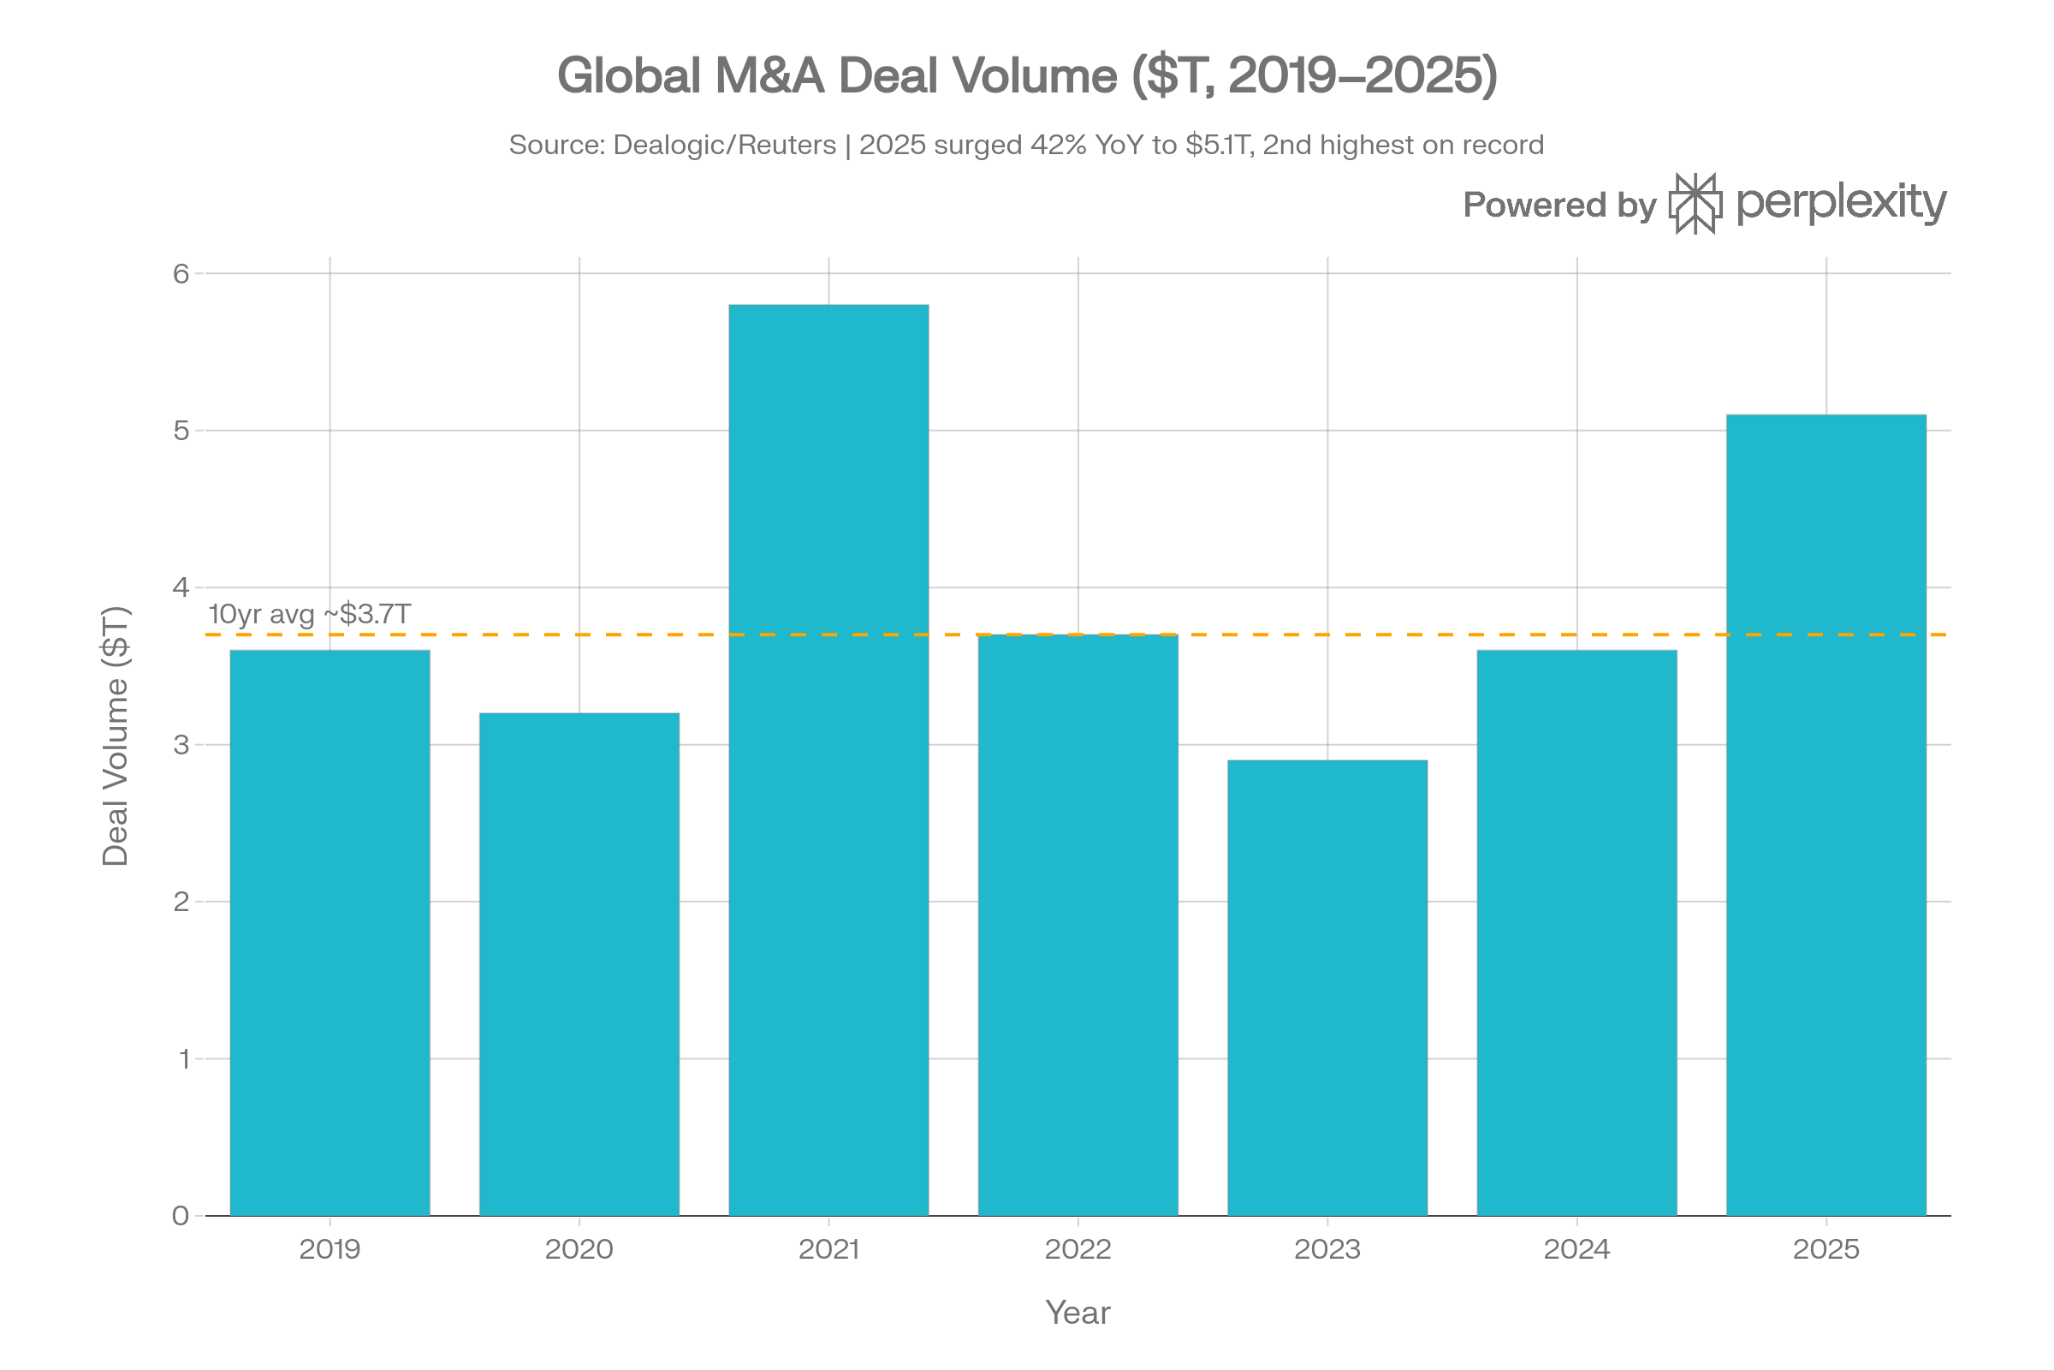
\includegraphics[height=0.52\textheight,keepaspectratio]{figures/slide42_img_flat.png}
\end{figure}
\end{column}
\end{columns}
\end{frame}

% [src: 43]
\begin{frame}{Deal Valuation Methodologies}
Investment bankers regularly employ three core approaches --- always used in combination (a ``football field''):
\begin{description}
  \item[Discounted cash flow (DCF)] Projects free cash flows and discounts them at the WACC
  \item[Comparable company analysis (``comps'')] Applies trading multiples (EV/EBITDA, P/E, P/S) from public peers to the target; adjustments for size, growth, and liquidity are critical
  \item[Precedent transaction analysis] Uses acquisition premiums and multiples from prior M\&A deals; typically yields \emph{higher} valuations than comps due to control premiums (historically averaging 25--35\%)
\end{description}
\end{frame}

% [src: 44]
\begin{frame}{Equity Capital Markets (ECM)}
ECM groups bridge corporate clients seeking equity financing with institutional investors.
\begin{itemize}
  \item ECM bankers manage the \textbf{book-building} process --- building an order book from institutional investors --- and price shares in a \textbf{roadshow}
  \item Relationships with buy-side accounts (mutual funds, hedge funds, pension funds) and the ability to manage price discovery are critical competitive advantages
  \item Two methods for the IPO process: \textbf{best efforts} and \textbf{firm commitment} (worked example next)
\end{itemize}
\end{frame}

% [src: 45]
\begin{frame}{Best Efforts vs.\ Firm Commitment: Example (1/3)}
An investment bank underwrites \textbf{20{,}000{,}000 shares} of Murray Construction Corp.\ on a \textbf{firm commitment} basis: the bank pays \$15.50 per share to Murray and sells to the public at \$16.35. \textbf{Profit to the bank?}
\[
\text{Profit} = (\$16.35 - \$15.50) \times 20{,}000{,}000 = \$17{,}000{,}000
\]
From Murray Construction's perspective, the \$17{,}000{,}000 is the \textbf{commission} it pays to issue the stock.
\end{frame}

% [src: 46, 47]
\begin{frame}{Best Efforts vs.\ Firm Commitment: Example (2/3)}
\textbf{Firm commitment downside:} if the bank can only sell at \$14.75:
\[
\text{Murray receives } \$15.50 \times 20{,}000{,}000 = \$310{,}000{,}000
\]
\[
\text{Bank profit} = (\$14.75 - \$15.50) \times 20{,}000{,}000 = -\$15{,}000{,}000
\]
--- the \textbf{risk} of the firm commitment.
\vspace{0.2em}

\textbf{Best efforts instead:} the bank sells 18{,}400{,}000 shares at \$15.50 and charges Murray \$0.375 per share sold. At \$15.50:
\[
\text{Murray receives } (\$15.50 - \$0.375) \times 18{,}400{,}000 = \$278{,}300{,}000
\]
\[
\text{Bank profit} = \$0.375 \times 18{,}400{,}000 = \$6{,}900{,}000
\]
\textbf{If shares sell at only \$14.75:} Murray receives $(\$14.75 - \$0.375) \times 18{,}400{,}000 = \$264{,}500{,}000$ --- but the bank's profit is \emph{still} \$6{,}900{,}000.
\end{frame}

% [src: 48]
\begin{frame}{Debt Capital Markets (DCM)}
DCM covers multiple markets simultaneously:
\begin{description}
  \item[Investment-grade corporate bonds] Lower yield, tighter spreads; dominated by BofA, JPMorgan, Citi
  \item[High-yield (``junk'') bonds] Higher yield; issuance rebounded strongly in 2024--2025 after the 2022--23 drought
  \item[Leveraged loans / CLOs] Floating-rate instruments integral to leveraged buyouts
  \item[ABS and CMBS] Securitized pools of mortgages, auto loans, or commercial real estate
\end{description}
\vspace{0.2em}
Banks sit at the intersection of trading floors and corporate coverage --- understanding investor demand and issuer needs simultaneously.
\end{frame}

% [src: 49]
\begin{frame}{Sales \& Trading}
\begin{itemize}
  \item Help execute trades of securities; provide investment research to clients (e.g., analyst reports)
  \item \textbf{Prime brokerage}: helping hedge funds trade, get leverage, locate shares for shorting, advise on trading ideas
\end{itemize}
\begin{center}
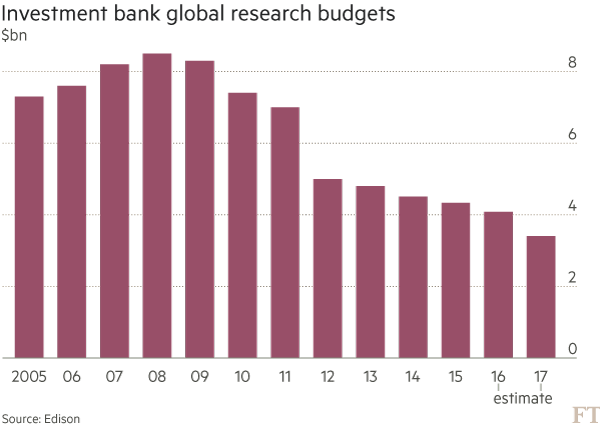
\includegraphics[height=0.34\textheight,keepaspectratio]{figures/slide49_img_flat.png}
\hspace{0.4em}
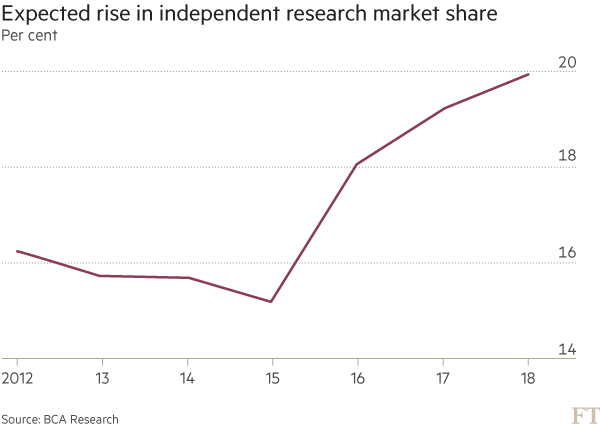
\includegraphics[height=0.34\textheight,keepaspectratio]{figures/slide49_img1_flat.png}
\end{center}
\note{Source of analyst chart: FT, 8 Feb 2017, ``Final call for the research analyst?'' (ft.com/content/85ee225a-ec4e-11e6-930f-061b01e23655).}
\end{frame}

% [src: 50, 51]
\begin{frame}{Research --- and Trading Revenues}
\textbf{Research} sits at the center of an information network: serving \emph{clients} (institutional investors), the \emph{media}, \emph{information providers}, and drawing on \emph{industry sources}, alongside CFE (certified financial examiners) and client interactions.
\vspace{0.3em}
\begin{description}
  \item[``Flow'' trading] Client-driven revenues --- fees, commissions, markups, and spreads measured through sales and production credits
  \item[``Prop'' trading] Risk-driven revenues --- dedicated proprietary trading delinked from customer business
\end{description}
\vspace{0.2em}
For most players, capital markets are primarily a \emph{client} business, not a proprietary trading business --- client franchise building is critical. The \textbf{Volcker rule} (part of the Dodd-Frank Act) prohibits prop trading in banks in the US.
\end{frame}

% [src: 52]
\begin{frame}{Career Paths and Compensation}
Investment banking offers some of the highest entry-level compensation in any profession; the hierarchy is steep, standardized, and performance-driven.
\begin{itemize}
  \item Typical path: \textbf{Analyst $\rightarrow$ Associate $\rightarrow$ VP $\rightarrow$ Director/ED $\rightarrow$ Managing Director}
  \item Most analysts join from undergraduate programs, spend 2--3 years, then exit to private equity, hedge funds, or an MBA with re-entry at Associate level
\end{itemize}
\begin{figure}
\centering
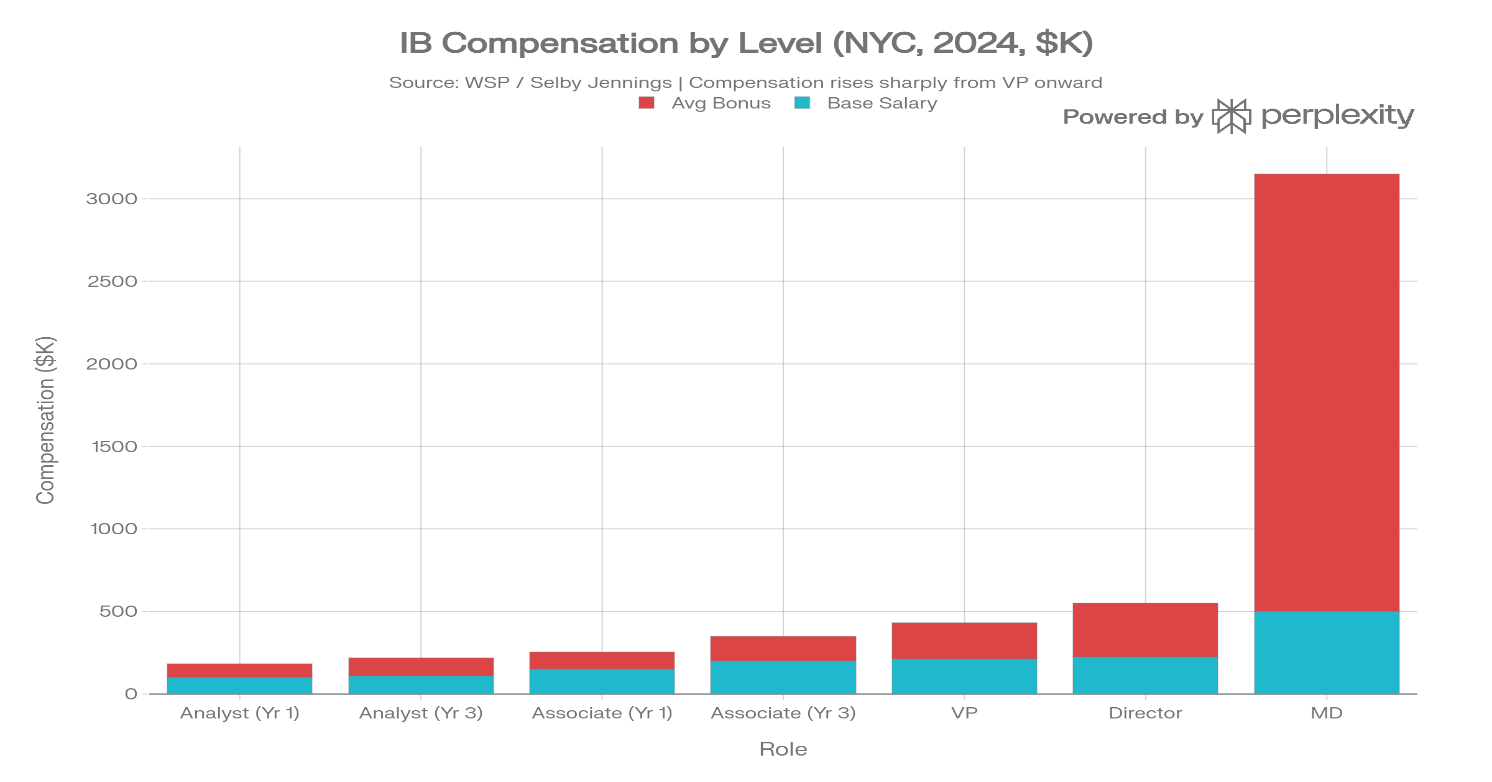
\includegraphics[height=0.44\textheight,keepaspectratio]{figures/slide52_img_flat.png}
\end{figure}
\note{Sources: Wall Street Prep, Selby Jennings, CFI. Elite boutiques (Evercore, Centerview) sometimes pay above bulge-bracket levels for analysts and associates.}
\end{frame}

% [src: 53]
\begin{frame}{Technology and AI Transformation}
AI is reshaping investment banking from front-office deal origination to back-office compliance:
\begin{itemize}
  \item Real-time transaction monitoring and fraud detection (JPMorgan reports a 20\% reduction in payment validation rejection rates)
  \item Automated credit underwriting and due diligence
  \item Equity research synthesis and earnings analysis
  \item Client segmentation and pitch book generation
  \item Risk model construction and regulatory reporting
\end{itemize}
\vspace{0.2em}
AI does not eliminate the investment banker; it eliminates the \textbf{junior tasks} that once justified entry-level positions. Develop judgment on complex, ambiguous problems, client relationship skills, and the ability to critically interpret AI outputs --- not just Excel modeling.
\end{frame}

% ============ IB REGULATION ============

% [src: 54]
\section{Regulation of the Investment Banking Industry}

% [src: 55]
\begin{frame}{Current Regulatory Environment}
\begin{itemize}
  \item Post-2008, the Basel III framework dramatically increased capital requirements --- banks now maintain CET1 ratios of no less than 12\%
  \item \textbf{Basel III Endgame re-proposed (March 19, 2026)}: the July 2023 proposal is dead; the re-proposal applies the expanded risk-based approach only to the largest banks (Category I--II, $\approx$8 US G-SIBs) and would \emph{reduce} aggregate CET1 requirements for those firms by $\approx$4.8\% (comment period closed June 18, 2026; final rule targeted for end-2026)
  \item The \textbf{eSLR} was finalized separately and took effect April 1, 2026 --- recalibrated to 50\% of the Method 1 G-SIB surcharge (bank-subsidiary cap 1\%), restoring it as a backstop rather than a binding constraint
  \item \textbf{G-SIB surcharge}: reform proposed March 2026 (not final); 29 G-SIBs worldwide in the FSB 2025 list, 8 of them US --- surcharge buckets 1.0\%--2.5\% (JPMorgan highest at 2.5\%)
\end{itemize}
\end{frame}

% [src: 56]
\begin{frame}{Investment Banks \& Commercial Banks}
\begin{itemize}
  \item Investment banks were essentially created in the US by the \textbf{Glass-Steagall Act (1933)}; before that, investment banking activities were part of large, money-center commercial banks
  \item As a result, J.P.\ Morgan \& Co.\ was broken up --- its investment banking activities spun off into \textbf{Morgan Stanley}
  \item The lines between investment and commercial banks began to blur again in the 1980s
  \item After the \textbf{Citi--Travellers merger (1998)}, the \textbf{Gramm-Leach-Bliley Act (1999)} (Financial Services Modernization Act) effectively repealed Glass-Steagall
\end{itemize}
\end{frame}

% [src: 57]
\begin{frame}{Framework for the Banking \& Securities Industry}
\begin{description}
  \item[Universal banking] Banks provide a full range of financial services (insurance, securities, real estate) under the same legal entity
  \item[Legal separation] Banks are prohibited from engaging in other financial services such as securities issuance and insurance
  \item[Financial supermarket (FHCs/BHCs)] Full range of services, but each activity under a different legal entity (subsidiary)
  \item[Global banks] Universal banking is more prevalent in Europe than the US --- e.g., Bank of America: commercial banking (BofA, N.A.), investment banking (BAML), wealth management (Merrill Lynch Wealth Management)
\end{description}
\note{Spurred by Gramm-Leach-Bliley (1999), many leading financial services companies now do business across sectors. GLB permits banks, securities firms, and insurance companies to affiliate through the financial holding company (FHC) structure; FHCs can engage in non-banking activities subject to Federal Reserve approval.}
\end{frame}

% [src: 58]
\begin{frame}{Should Glass-Steagall Be Reinstated?}
\begin{columns}
\begin{column}{0.48\textwidth}
\textbf{Pros}
\begin{itemize}
  \item Protect depositors
  \item Simplify regulation of depository institutions
  \item More transparency for depository institutions' customers
  \item Lessens systemic risk and limits financial-risk contagion
\end{itemize}
\end{column}
\begin{column}{0.48\textwidth}
\textbf{Cons}
\begin{itemize}
  \item Restricts financial innovation
  \item Limits profit opportunity and competition
  \item Banks will find other loopholes, just like in the past
\end{itemize}
\end{column}
\end{columns}
\end{frame}

% [src: 59, 60]
\begin{frame}{Key Takeaways}
\begin{itemize}
  \item \textbf{Commercial banks:} intermediaries taking deposits (liabilities) and issuing loans (assets); profit from the interest rate spread but face maturity mismatch and liquidity risk
  \item \textbf{Bank regulation:} heavy regulation for stability and depositor protection --- FDIC (deposit insurance), the Fed, the OCC; minimum equity capital buffers losses
  \item \textbf{Investment banks:} operate primarily in capital markets --- underwriting new securities (debt/equity) and M\&A advisory; revenue from fees, commissions, and trading spreads
  \item \textbf{Two ways to underwrite:} firm commitment --- the bank bears the risk of unsold shares (buys the entire issue); best efforts --- the issuer bears the risk, the bank earns a commission on shares sold
  \item \textbf{Industry evolution:} Glass-Steagall (1933) separated commercial and investment banking; effectively repealed in 1999, enabling financial conglomerates (BHCs, FHCs) offering both under one umbrella
\end{itemize}
\end{frame}

\end{document}
